\subsection{Динамика манипулятора}\label{part_dynamics}

\subsubsection{Общие замечания}
Введем в рассмотрение барицентрические СК $Ox_{ci}y_{ci}z_{ci}$\lefteqn,\footnote{Системы координат, чьи начала совпадают с центрами масс соответствующих звеньев.} где $i=\overline{1,5}$, показанные на рисунке~\ref{img_mass_frames}.
Заметим, что каждая СК $Ox_{ci}y_{ci}z_{ci}$ сонаправлена с~$Ox_iy_iz_i$.

\begin{figure}[h!]
	\centering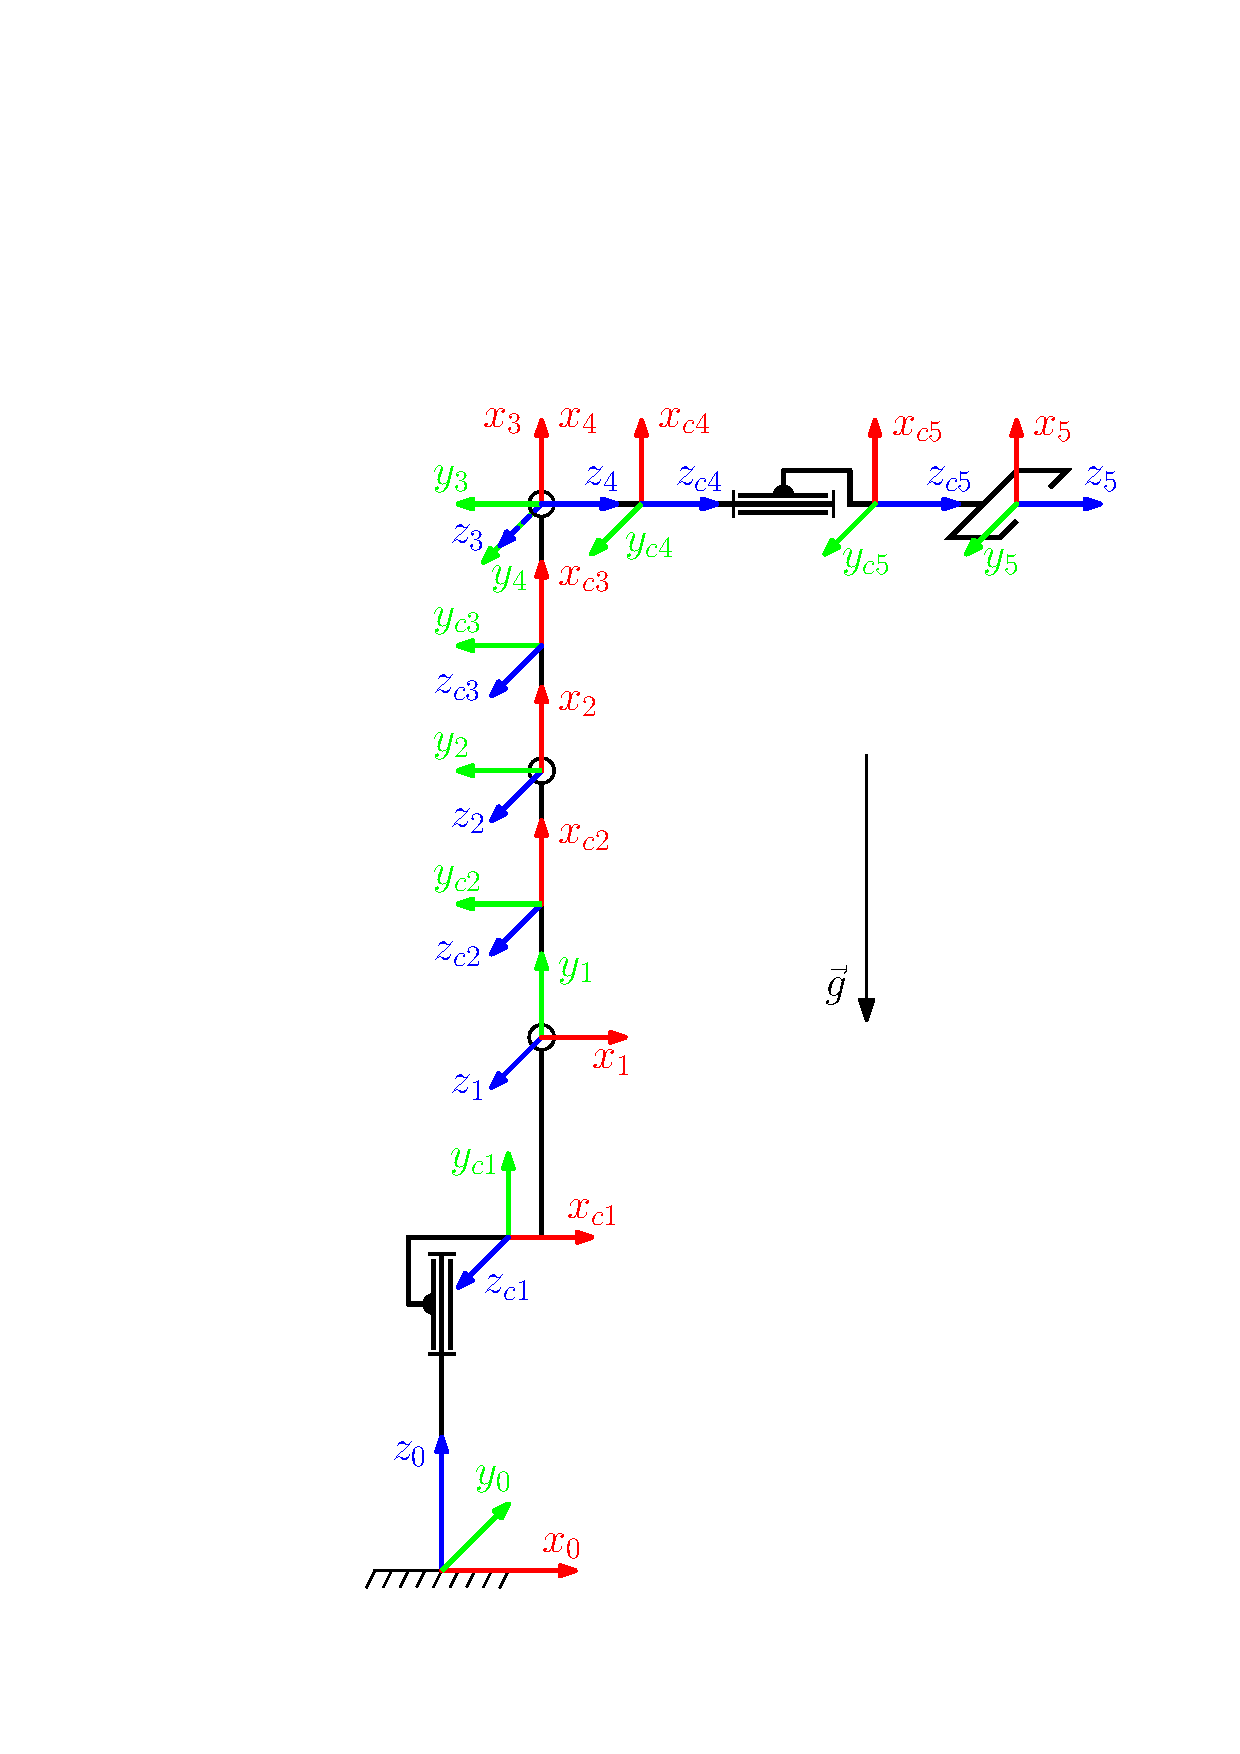
\includegraphics[height=16.5cm]{kinematics_mass_frames.pdf}
	\caption{Положение барицентрических СК и направление вектора $\vec{g}$.}
	\label{img_mass_frames}
\end{figure}

Для описания положения введенных СК воспользуемся следующими векторами:
\begin{equation}
    r^i_{i,\,ci} =
    \begin{bmatrix}
        x_{ci} \\ y_{ci} \\ z_{ci}
    \end{bmatrix}\!\!,\quad i = \overline{1,5},
\end{equation}
где $x_{ci}$, $y_{ci}$ и $z_{ci}$~--- некоторые постоянные величины.

Для компонент тензоров инерции $\mathcal{I}^{i}_i = const$ введем следующие обозначения:
\begin{equation}
    \mathcal{I}^{i}_i =
    \begin{bmatrix}
        I_{i,\,xx} & I_{i,\,xy} & I_{i,\,xz} \\
        I_{i,\,xy} & I_{i,\,yy} & I_{i,\,yz} \\
        I_{i,\,xz} & I_{i,\,yz} & I_{i,\,zz}
    \end{bmatrix}\!\!\ldotp
\end{equation}

Заметим, что
\begin{equation}
    g_0 =
    \begin{bmatrix}
        0 \\ 0 \\ -g
    \end{bmatrix}\!\!,
\end{equation}
где $g=9.82\text{ м}/\text{с}^2$.

В~заключении раздела приведем формулы для расчета величин, которые потребуются в дальнейшем (везде $i = \overline{1,5}$):
\begin{itemize}
    \item для расчета $r^0_{0,\,i}$ и ${}^{0}R_i$ (см.~Приложение~\ref{app_ht_matrices}):
        \begin{equation}
            {}^0A_i = {}^0A_1 \cdot {}^1A_2 \cdot \ldots \cdot {}^{i-1}A_i;
        \end{equation}
    \item для расчета $r^i_{0,\,i}$:
        \begin{gather}
            r^i_{0,\,i} = {}^{0}R_i^T \cdot r^0_{0,\,i};
        \end{gather}
    \item для расчета $z^0_i$:
        \begin{equation}
            z^0_i = {}^{0}R_i \cdot z^i_i = {}^{0}R_i \cdot
            \begin{bmatrix}
                0 \\ 0 \\ 1
            \end{bmatrix}\!\!;
        \end{equation}
    \item для расчета $g_i$, $v^i_i$ и $\omega^i_i$:
        \begin{equation}\label{eq_transform_of_g_v_omega}
            g_i = {}^{0}R_i^T \cdot g_0,
            \qquad
            v^i_i = {}^{0}R_i^T \cdot v^0_i,
            \qquad
            \omega^i_i = {}^{0}R_i^T \cdot \omega^0_i \ldotp
        \end{equation}
\end{itemize}

\subsubsection{Вывод уравнений движения}
Потенциальная энергия манипулятора
\begin{equation}
    U =  -\sum_{i=1}^5 \left( m_i g_i^T r^i_{0,\,ci} \right) = -\sum_{i=1}^5 \left( m_i g_i^T r^i_{0,\,i} + g_i^T (m_ir^i_{i,\,ci}) \right)\!,
\end{equation}


Якобианы, устанавливающие в соответствии с формулой
\begin{equation}\label{eq_work_of_lin_jacobians}
    v^0_{i} = -J_{vi}\dot{q}, \quad i = \overline{1,5}
\end{equation}
связь между линейными скоростями начал соответствующих СК и вектором~$\dot{q}$:
\begin{gather}
    J_{v1} =
    \begin{bmatrix}
        z^0_0 \times \left( r^0_{0,\,1} - r^0_{0,\,0}\right) & \nv & \nv & \nv & \nv
    \end{bmatrix}\!\!,
    \\
    J_{v2} =
    \begin{bmatrix}
        z^0_0 \times \left( r^0_{0,\,2} - r^0_{0,\,0}\right) & z^0_1 \times \left( r^0_{0,\,2} - r^0_{0,\,1}\right) & \nv & \nv & \nv
    \end{bmatrix}\!\!,
    \\
    J_{v3} =
    \begin{bmatrix}
        z^0_0 \times \left( r^0_{0,\,3} - r^0_{0,\,0}\right) & z^0_1 \times \left( r^0_{0,\,3} - r^0_{0,\,1}\right) &
        z^0_2 \times \left( r^0_{0,\,3} - r^0_{0,\,2}\right) & \nv & \nv
    \end{bmatrix}\!\!,
    \\
    J_{v4} =
    \begin{bmatrix}
        z^0_0 \times \left( r^0_{0,\,4} - r^0_{0,\,0}\right) \\
        z^0_1 \times \left( r^0_{0,\,4} - r^0_{0,\,1}\right) \\
        z^0_2 \times \left( r^0_{0,\,4} - r^0_{0,\,2}\right) \\
        z^0_3 \times \left( r^0_{0,\,4} - r^0_{0,\,3}\right) \\
        \nv
    \end{bmatrix}^T\!\!\!\!\!,
    \qquad
    J_{v5} =
    \begin{bmatrix}
        z^0_0 \times \left( r^0_{0,\,5} - r^0_{0,\,0}\right) \\
        z^0_1 \times \left( r^0_{0,\,5} - r^0_{0,\,1}\right) \\
        z^0_2 \times \left( r^0_{0,\,5} - r^0_{0,\,2}\right) \\
        z^0_3 \times \left( r^0_{0,\,5} - r^0_{0,\,3}\right) \\
        z^0_4 \times \left( r^0_{0,\,5} - r^0_{0,\,4}\right)
    \end{bmatrix}^T\!\!\!\!\!,
\end{gather}
где $\nv = [0\;0\;0]^T$~--- нулевой вектор.

Якобианы, устанавливающие в соответствии с формулой
\begin{equation}\label{eq_work_of_ang_jacobians}
    \omega^0_{i} = -J_{\omega i}\dot{q}, \quad i = \overline{1,5}
\end{equation}
связь между угловыми скоростями звеньев и вектором~$\dot{q}$:
\begin{gather}
    J_{\omega 1} =
    \begin{bmatrix}
        z^0_0 & \nv & \nv & \nv & \nv
    \end{bmatrix}\!\!,
    \qquad
    J_{\omega 2} =
    \begin{bmatrix}
        z^0_0 & z^0_1 & \nv & \nv & \nv
    \end{bmatrix}\!\!,
    \\
    J_{\omega 3} =
    \begin{bmatrix}
         z^0_0 & z^0_1 & z^0_2 & \nv & \nv
    \end{bmatrix}\!\!,
    \qquad
    J_{\omega 4} =
    \begin{bmatrix}
        z^0_0 & z^0_1 & z^0_2 & z^0_3 & \nv
    \end{bmatrix}\!\!,
    \\
    J_{\omega 5} =
    \begin{bmatrix}
        z^0_0 & z^0_1 & z^0_2 & z^0_3 & z^0_4
    \end{bmatrix}\!\!\ldotp
\end{gather}

Кинетическая энергия манипулятора
\begin{equation}\label{eq_eq_for_K_for_linear_model}
    K = \sum_{i=1}^5 \left( \frac{1}{2} m_i (v^i_i)^T v^i_i + \frac{1}{2} (\omega^i_i)^T \mathcal{I}^{i}_i \omega^i_i + (m_ir^i_{i,\,ci})^T \cdot (v^i_i \times \omega^i_i) \right)  \ldotp
\end{equation}

Функция Лагранжа
\begin{gather}
    L = K - U = \notag
    \\
    = \sum_{i=1}^5 \Biggl( m_i \left( \frac{1}{2} (v^i_i)^T v^i_i + g_i^T r^i_{0,\,i} \right) + (m_ir^i_{i,\,ci})^T \cdot \left( v^i_i \times \omega^i_i + g_i \right) + \frac{1}{2} (\omega^i_i)^T \mathcal{I}^{i}_i \omega^i_i \Biggr) = \notag
    \\
    = \sum_{i=1}^5 \Biggl( m_i \underbrace{\left( \frac{1}{2} (v^i_i)^T v^i_i + g_i^T r^i_{0,\,i} \right)}_{\ds L_{i,1}} + m_i x_{ci} \cdot \underbrace{x\left\{ v^i_i \times \omega^i_i + g_i \right\}}_{\ds L_{i,2}} + \notag
    \\
    + m_i y_{ci} \cdot \underbrace{y\left\{ v^i_i \times \omega^i_i + g_i \right\}}_{\ds L_{i,3}} + m_i z_{ci} \cdot \underbrace{z\left\{ v^i_i \times \omega^i_i + g_i \right\}}_{\ds L_{i,4}} + I_{i,\,xx} \cdot \underbrace{\frac{1}{2} \cdot \bigl(x\{\omega^i_i\}\bigr)^2}_{\ds L_{i,5}} +\notag
    \\
    + I_{i,\,yy} \cdot \underbrace{\frac{1}{2} \cdot \bigl(y\{\omega^i_i\}\bigr)^2}_{\ds L_{i,6}} + I_{i,\,zz} \cdot \underbrace{\frac{1}{2} \cdot \bigl(z\{\omega^i_i\}\bigr)^2}_{\ds L_{i,7}} + I_{i,\,xy} \cdot \underbrace{x\{\omega^i_i\} \cdot y\{\omega^i_i\}}_{\ds L_{i,8}} +\notag
    \\
    + I_{i,\,xz} \cdot \underbrace{x\{\omega^i_i\} \cdot z\{\omega^i_i\}}_{\ds L_{i,9}} + I_{i,\,yz} \cdot \underbrace{y\{\omega^i_i\} \cdot z\{\omega^i_i\}}_{\ds L_{i,10}}\Biggr) \ldotp
\end{gather}

Уравнения движения робота:
\begin{equation}
    \frac{d}{dt}\frac{\partial L}{\partial\dot{q_i}} - \frac{\partial L}{\partial q_i} = \tau_i, \quad i = \overline{1,5} \qquad \Rightarrow
\end{equation}
\begin{equation}
    \Rightarrow \quad
	\left\{
	\begin{aligned}
		\!&\sum_{i=1}^5 \bigl( m_i \cdot \mathcal{L}_1 \{L_{i,1}\} + m_i x_{ci} \cdot \mathcal{L}_1 \{L_{i,2}\} + \ldots + I_{i,\,yz} \cdot \mathcal{L}_1 \{L_{i,10}\} \bigr) = \tau_1\\
		\!&\sum_{i=1}^5 \bigl( m_i \cdot \mathcal{L}_2 \{L_{i,1}\} + m_i x_{ci} \cdot \mathcal{L}_2 \{L_{i,2}\} + \ldots + I_{i,\,yz} \cdot \mathcal{L}_2 \{L_{i,10}\} \bigr) = \tau_2\\
		\!&\ldots\\
		\!&\sum_{i=1}^5 \bigl( m_i \cdot \mathcal{L}_5 \{L_{i,1}\} + m_i x_{ci} \cdot \mathcal{L}_5 \{L_{i,2}\} + \ldots + I_{i,\,yz} \cdot \mathcal{L}_5 \{L_{i,10}\} \bigr) = \tau_5
	\end{aligned}
	\right.
\end{equation}
где $\mathcal{L}_j$~--- оператор, работающий в соответствии с формулой:
\begin{equation}
    \mathcal{L}_j : \quad \mathcal{L}_j \{f\} = \frac{d}{dt}\frac{\partial f}{\partial\dot{q_j}} - \frac{\partial f}{\partial q_j},
\end{equation}
где в свою очередь $f = f(\dot{q}(t), q(t))$.
Если же заметить, что
\begin{equation}
    \mathcal{L}_j \{L_{i,k}\} = 0 \qquad \text{при }j > i, \quad i,j=\overline{1,5}, \quad k=\overline{1,10},
\end{equation}
то выражения для них упрощаются до:
\begin{equation}
	\left\{
	\begin{aligned}
		\!&\sum_{i=1}^5 \bigl( m_i \cdot \mathcal{L}_1 \{L_{i,1}\} + m_i x_{ci} \cdot \mathcal{L}_1 \{L_{i,2}\} + \ldots + I_{i,\,yz} \cdot \mathcal{L}_1 \{L_{i,10}\} \bigr) = \tau_1\\
		\!&\sum_{i=2}^5 \bigl( m_i \cdot \mathcal{L}_2 \{L_{i,1}\} + m_i x_{ci} \cdot \mathcal{L}_2 \{L_{i,2}\} + \ldots + I_{i,\,yz} \cdot \mathcal{L}_2 \{L_{i,10}\} \bigr) = \tau_2\\
		\!&\ldots\\
		\!& m_5 \cdot \mathcal{L}_5 \{L_{5,1}\} + m_5 x_{c5} \cdot \mathcal{L}_5 \{L_{5,2}\} + \ldots + I_{5,\,yz} \cdot \mathcal{L}_5 \{L_{5,10}\} = \tau_5
	\end{aligned}
	\right.
\end{equation}
или в матричном виде
\begin{equation}\label{eq_dynamic_in_linear}
    \tau = \xi \chi,
\end{equation}
где $\tau = [\tau_1, \: \tau_2, \: \ldots, \: \tau_5]^T$~--- вектор обобщенных моментов,\\ $\chi=[\chi_1, \: \chi_2, \: \ldots, \: \chi_5]^T \in \mathbb R^{50}$~--- вектор параметров робота, где в свою очередь
\begin{equation}
    \chi_i =
    \begin{bmatrix}
        m_i & m_i x_{ci} & m_i y_{ci} & m_i z_{ci} & I_{i,\,xx} & I_{i,\,yy} & I_{i,\,zz} & I_{i,\,xy} & I_{i,\,xz} & I_{i,\,yz}
    \end{bmatrix}^T\!\!\!\!;
\end{equation}
$\xi$~--- так называемый регрессор, равный
\begin{equation}
    \xi =
    \begin{bmatrix}
        \xi_{1,1} & \xi_{1,2} & \cdots & \xi_{1,5} \\
        O_{1 \times 10} & \xi_{2,2} & \cdots & \xi_{2,5} \\
        \vdots & \vdots & \ddots & \vdots \\
        O_{1 \times 10} & O_{1 \times 10} & O_{1 \times 10} & \xi_{5,5}
    \end{bmatrix}\!\!,
\end{equation}
где в свою очередь $O_{1 \times 10}$~--- вектор-строка, состоящая из 10 нулей, а $\xi_{j,i} =$\linebreak $= \xi_{j,i}(\ddot{q}, \dot{q}, q)$~--- вектор-строка, рассчитываемый по формуле
\begin{equation}
    \xi_{j,i} =
    \begin{bmatrix}
        \mathcal{L}_j \{L_{i,1}\} & \mathcal{L}_j \{L_{i,2}\} & \ldots & \mathcal{L}_j \{L_{i,10}\}
    \end{bmatrix}\!\!\ldotp
\end{equation}

\subsubsection{Учет динамики приводов}
Уравнения, описывающие динамику приводов, в матричном виде имеют вид
\begin{equation}\label{eq_actuators_dynamic}
    I_a \ddot{q} = \tau_e - \tau,
\end{equation}
где $I_a$~--- диагональная матрица приведенных к выходным валам моментов инерции приводов, $\tau_e$~--- вектор-столбец приведенных к выходным валам приводов моментов силы, развиваемых двигателями, имеющие вид:
\begin{equation}
    I_a =
    \begin{bmatrix}
        I_{a,1} & 0 & \cdots & 0 \\
        0 & I_{a,2} & \cdots & 0 \\
        \vdots & \vdots & \ddots & 0 \\
        0 & 0 & \cdots & I_{a,5}
    \end{bmatrix}\!\!,
    \qquad \qquad
    \tau_e =
    \begin{bmatrix}
        \tau_{e,1} \\ \tau_{e,2} \\ \vdots \\ \tau_{e,5}
    \end{bmatrix}\!\!\ldotp
\end{equation}

Объединяя уравнения~\eqref{eq_dynamic_in_linear} и~\eqref{eq_actuators_dynamic}, получим
\begin{equation}
    \tau_e = I_a \ddot{q} + \xi \chi,
\end{equation}
а, добавив в это выражение учет моментов трения, окончательно будем иметь
\begin{equation}\label{eq_eqs_with_tau_f}
    \tau_e = I_a \ddot{q} + \xi \chi + t_f \ldotp
\end{equation}

В~качестве модели трения возьмем поясняемую рисунком~\ref{img_friction_torque} и описываемую следующим уравнением
\begin{equation}\label{eq_friction_torque}
    \tau_f(\dot{q}) = f_v \dot{q} + f_c \sign(\dot{q}) + f_\text{off},
\end{equation}
где $f_v$, $f_c$~--- диагональные матрицы коэффициентов вязкого и сухого трения соответственно, $f_\text{off}$~--- вектор-столбец сдвигов в моментах силы, имеющие вид
\begin{equation}
    f_v =
    \begin{bmatrix}
        f_{v,1} & 0 & \cdots & 0 \\
        0 & f_{v,2} & \cdots & 0 \\
        \vdots & \vdots & \ddots & 0 \\
        0 & 0 & \cdots & f_{v,5}
    \end{bmatrix}\!\!,
    \quad
    f_c =
    \begin{bmatrix}
        f_{c,1} & 0 & \cdots & 0 \\
        0 & f_{c,2} & \cdots & 0 \\
        \vdots & \vdots & \ddots & 0 \\
        0 & 0 & \cdots & f_{c,5}
    \end{bmatrix}\!\!,
    \quad
    f_\text{off} =
    \begin{bmatrix}
        f_{\text{off},1} \\ f_{\text{off},2} \\ \vdots \\ f_{\text{off},5}
    \end{bmatrix}\!\!\ldotp
\end{equation}

\begin{figure}[h!]
	\centering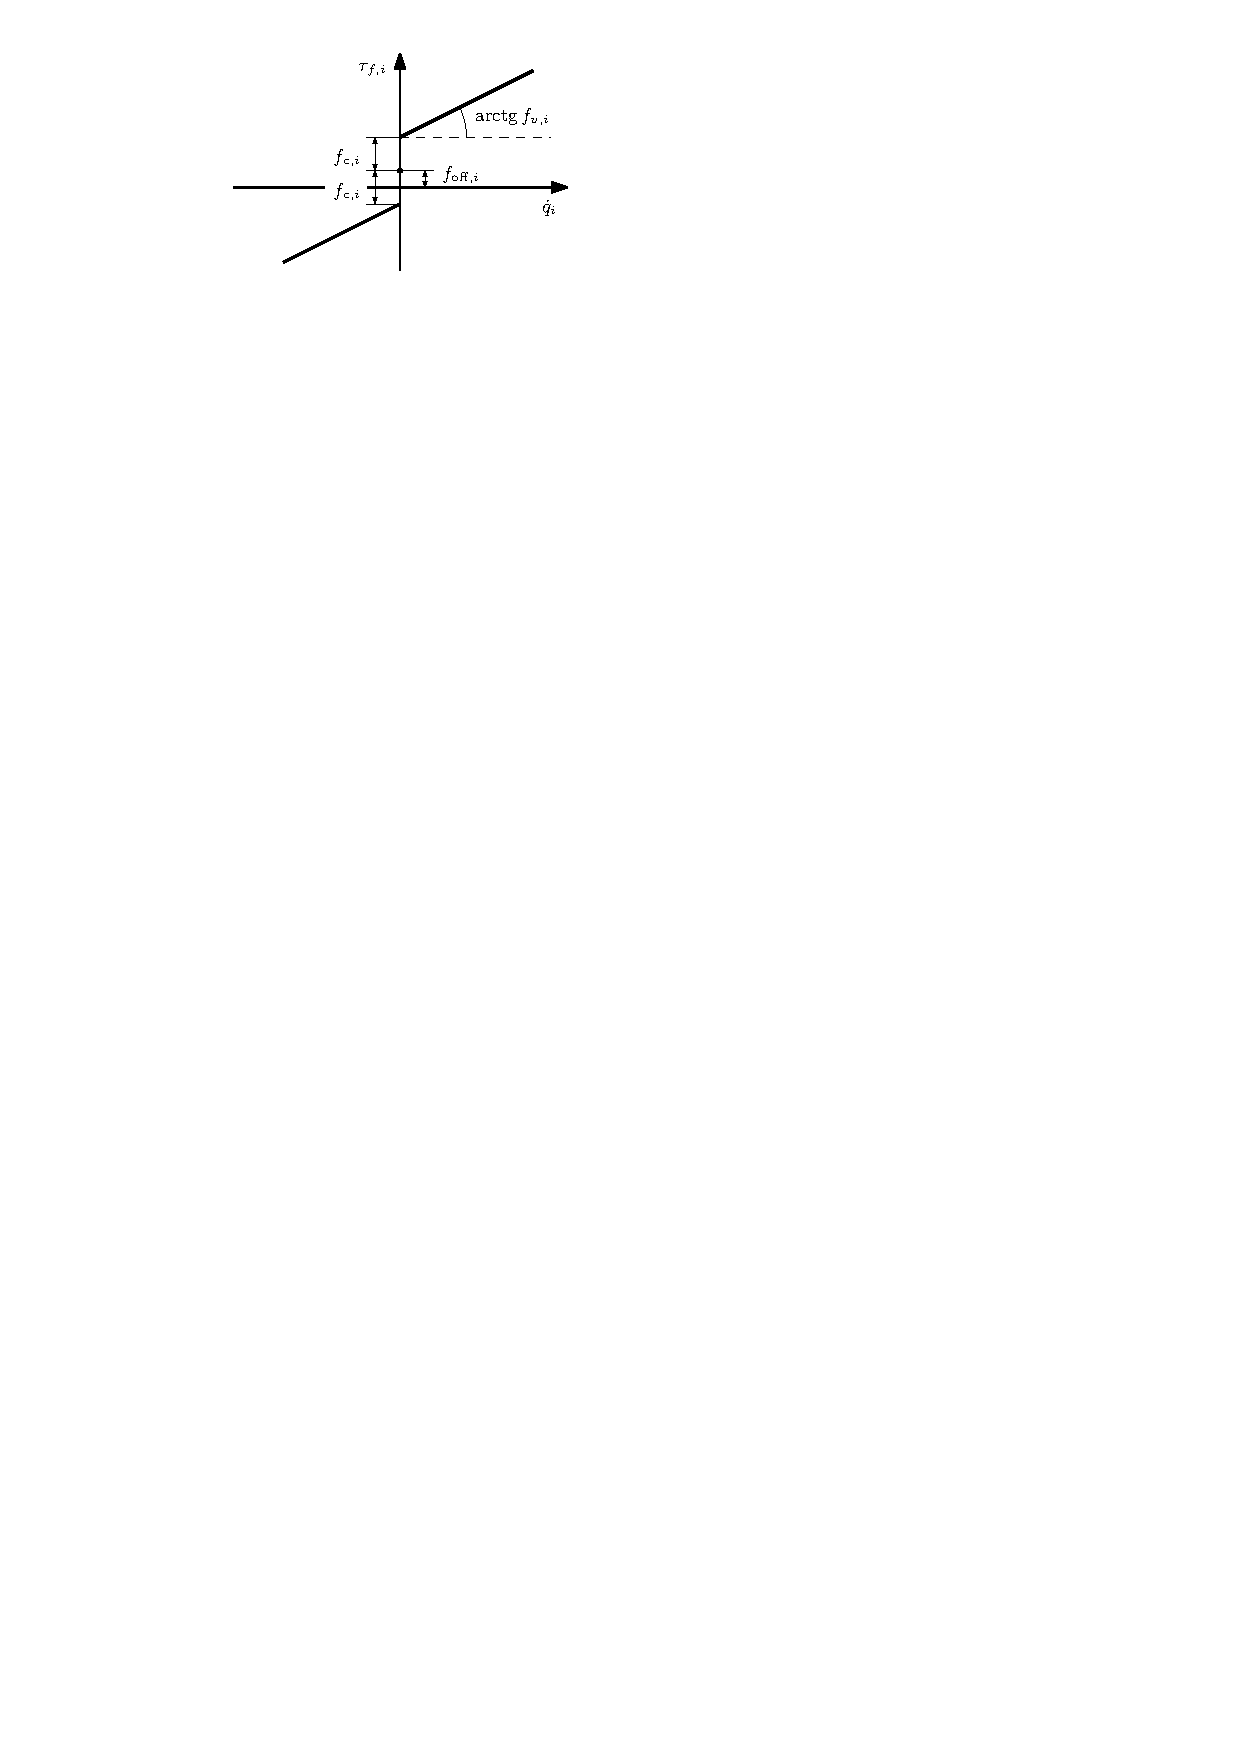
\includegraphics[width=0.7\textwidth]{friction_torque.pdf}
	\caption{График, поясняющий выбранную модель трения.}
	\label{img_friction_torque}
\end{figure}

Подставляя~\eqref{eq_friction_torque} в~\eqref{eq_eqs_with_tau_f}, получим
\begin{equation}
     \tau_e = I_a \ddot{q} + \xi \chi + f_v \dot{q} + f_c \sign(\dot{q}) + f_\text{off}\ldotp
\end{equation}
Если ввести в рассмотрение новые матрицы $\bar{\chi}=[\bar{\chi}_1, \: \bar\chi_2, \: \ldots, \: \bar\chi_5]^T$ и\linebreak
\begin{equation}
    \bar\xi =
    \begin{bmatrix}
        \bar\xi_{1,1} & \bar\xi_{1,2} & \cdots & \bar\xi_{1,5} \\
        O_{1 \times 10} & \bar\xi_{2,2} & \cdots & \bar\xi_{2,5} \\
        \vdots & \vdots & \ddots & \vdots \\
        O_{1 \times 10} & O_{1 \times 10} & O_{1 \times 10} & \bar\xi_{5,5}
    \end{bmatrix}\!\!,
\end{equation}
определяемые выражениями
\begin{equation}
    \bar{\chi}_i =
    \begin{bmatrix}
        \chi_i & I_{a,i} & f_{v,i} & f_{c,i} & f_{\text{off},i}
    \end{bmatrix}^T\!\!\!\!,
\end{equation}
\begin{equation}
    \bar{\xi}_{j,i} =
    \left\{
    \begin{aligned}
        \!\begin{bmatrix}\xi_{j,i} & 0 & 0 & 0 & 0\end{bmatrix}&, && i \ne j \\
        \!\begin{bmatrix}\xi_{j,i} & \ddot{q_j} & \dot{q_j} & \sign(\dot{q_j}) & 1\end{bmatrix}&, &&i = j
	\end{aligned}
	\right.
\end{equation}
то данное выражение может быть записано в следующем матричном виде:
\begin{equation}\label{eq_extended_dynamic_in_linear}
    \tau_e = \bar\xi \bar\chi \ldotp
\end{equation}

\subsubsection{Альтернативная матричная форма записи}\label{part_matrix_form_of_equation}
Выражение~\eqref{eq_dynamic_in_linear} может быть переписано в форме
\begin{equation}
    \tau = D(q) \ddot{q} + C(q,\dot{q}) \dot{q} + G(q),
\end{equation}
где $D(q)$~--- матрица инерции, $C(q,\dot{q})$~--- матрица центробежных и Кориолисовых сил, $G(q)$~--- вектор гравитации.
С~учетом этого факта и уравнения~\eqref{eq_eqs_with_tau_f} можно получить, что
\begin{equation}\label{eq_model_with_standard_matrix}
    \tau_e = M(q) \ddot{q} + C(q,\dot{q}) \dot{q} + G(q) + t_f(\dot{q}),
\end{equation}
где $M(q) = I_a + D(q)$.

Выражение для матрицы~$D(q)$ может быть найдено из формулы для кинетической энергии с учетом того, что справедливо
\begin{equation}\label{eq_K_in_form_with_D}
    \left\{
    \begin{aligned}
        \!& K = \frac{1}{2} \, \dot{q}^T D(q) \dot{q}, \\
        \!& D(q) = D^T\!(q),
    \end{aligned}
    \right.
\end{equation}
для матрицы $C(q,\dot{q})$~--- из выражения для $D(q)$ в соответствии с формулами:
\begin{gather}
    C_{ijk} = \cfrac{1}{2} \left( \cfrac{\partial D_{kj}}{\partial q_i} + \cfrac{\partial D_{ki}}{\partial q_j} - \cfrac{\partial D_{ij}}{\partial q_k}\right)\!\!,
    \\
    C_{kj} = \sum_{i = 1}^n C_{ijk} \dot{q}_i,
\end{gather}
где $D_{ij}$, $C_{ij}$~--- элементы матриц $D(q)$ и $C(q,\dot{q})$ соответственно, стоящие на пересечении $i$-ой строки и $j$-го столбца;
а для вектора $G(q)$~--- по формуле
\begin{equation}
    G(q) =
    \begin{bmatrix}
        \cfrac{\partial U}{\partial q_1} &
        \cfrac{\partial U}{\partial q_2} &
        \dots &
        \cfrac{\partial U}{\partial q_5}
    \end{bmatrix}^T\!\!\!\!\!\ldotp
\end{equation}

Выражение для кинетической энергии в форме, иллюстрируемой первым из уравнений~\eqref{eq_K_in_form_with_D}, может быть получено из уравнения~\eqref{eq_eq_for_K_for_linear_model} с учетом формул~\eqref{eq_transform_of_g_v_omega}, \eqref{eq_work_of_lin_jacobians} и \eqref{eq_work_of_ang_jacobians}:
\begin{gather}
    K = \sum_{i=1}^5 \biggl( \frac{1}{2} m_i \cdot \left( -{}^0R_i^T J_{vi} \dot{q} \right)^T \!\!\cdot \left(-{}^0R_i^T J_{vi} \dot{q}\right) + \frac{1}{2} \left( -{}^0R_i^T J_{\omega i} \dot{q} \right)^T \!\!\cdot \mathcal{I}^{i}_i \cdot \left( -{}^0R_i^T J_{\omega i} \dot{q} \right) + {}\notag\\
    %
    {} + (m_ir^i_{i,\,ci})^T \cdot \Bigl( \left( -{}^0R_i^T J_{vi} \dot{q} \right) \times \left( -{}^0R_i^T J_{\omega i} \dot{q} \right) \Bigr) \biggr) = {}\notag\\
    %
    {} = \sum_{i=1}^5 \biggl(\frac{1}{2} m_i \dot{q}^T J_{vi}^T J_{vi} \dot{q} \!+\! \frac{1}{2} \dot{q}^T J_{\omega i}^T \, {}^0\!R_i \, \mathcal{I}^{i}_i \, {}^0\!R_i^T J_{\omega i} \dot{q} \!+\! (m_i \underbrace{{}^0\!R_i r^i_{i,\,ci}}_{\displaystyle r^0_{i,\,ci}})^T \!\!\cdot \Bigl( \left( J_{vi} \dot{q} \right) \times \left( J_{\omega i} \dot{q} \right) \Bigr) \!\biggr) = {}\notag \\
    %
    {} = \frac{1}{2} \dot{q}^T \Biggl(\sum_{i=1}^5 \Bigl(m_i J_{vi}^T J_{vi} + J_{\omega i}^T \, {}^0\!R_i \, \mathcal{I}^{i}_i \, {}^0\!R_i^T J_{\omega i} + 2 \cdot x\{ m_i r^0_{i,\,ci} \} \!\cdot\! J_{xi}  + {}\notag \\
    %
    {} + 2 \cdot y\{ m_i r^0_{i,\,ci} \} \!\cdot\! J_{yi} + 2 \cdot z\{ m_i r^0_{i,\,ci} \} \!\cdot\! J_{zi}\Bigr) \Biggr) \dot{q}, \label{eq_getting_form_with_D_for_K}
\end{gather}
при преобразованиях которого учтено то, что
\begin{equation*}
    \left( J_{vi} \dot{q} \right) \times \left( J_{\omega i} \dot{q} \right) =
    \begin{bmatrix}
        J_{vi}^{\{1\}} \dot{q}\\
        J_{vi}^{\{2\}} \dot{q}\\
        J_{vi}^{\{3\}} \dot{q}
    \end{bmatrix}
    \times
    \begin{bmatrix}
        J_{\omega i}^{\{1\}} \dot{q}\\
        J_{\omega i}^{\{2\}} \dot{q}\\
        J_{\omega i}^{\{3\}} \dot{q}
    \end{bmatrix}
    =
    \begin{bmatrix}
        -J_{vi}^{\{3\}} \dot{q} J_{\omega i}^{\{2\}} \dot{q} + J_{vi}^{\{2\}} \dot{q} J_{\omega i}^{\{3\}} \dot{q}\\
         J_{vi}^{\{3\}} \dot{q} J_{\omega i}^{\{1\}} \dot{q} - J_{vi}^{\{1\}} \dot{q} J_{\omega i}^{\{3\}} \dot{q}\\
        -J_{vi}^{\{2\}} \dot{q} J_{\omega i}^{\{1\}} \dot{q} + J_{vi}^{\{1\}} \dot{q} J_{\omega i}^{\{2\}} \dot{q}
    \end{bmatrix}
    =
\end{equation*}
\begin{equation}
    =
    \begin{bmatrix}
        -\dot{q}^T \bigl(J_{vi}^{\{3\}} \bigr)^T J_{\omega i}^{\{2\}} \dot{q} +
        \dot{q}^T \bigl( J_{vi}^{\{2\}} \bigr)^T J_{\omega i}^{\{3\}} \dot{q}
        \\
        \dot{q}^T \bigl( J_{vi}^{\{3\}} \bigr)^T J_{\omega i}^{\{1\}} \dot{q} -
        \dot{q}^T \bigl( J_{vi}^{\{1\}} \bigr)^T J_{\omega i}^{\{3\}} \dot{q}
        \\
        -\dot{q}^T \bigl( J_{vi}^{\{2\}} \bigr)^T J_{\omega i}^{\{1\}} \dot{q} +
        \dot{q}^T \bigl( J_{vi}^{\{1\}} \bigr)^T J_{\omega i}^{\{2\}} \dot{q}
    \end{bmatrix}
    =
    \begin{bmatrix}
        \dot{q}^T \! J_{xi} \dot{q} \\
        \dot{q}^T \! J_{yi} \dot{q} \\
        \dot{q}^T \! J_{zi} \dot{q}
    \end{bmatrix}\!\!,
\end{equation}
где
\begin{align}
    &J_{xi} =  - \bigl( J_{vi}^{\{3\}} \bigr)^T J_{\omega i}^{\{2\}} + \bigl( J_{vi}^{\{2\}} \bigr)^T J_{\omega i}^{\{3\}}, \\
    &J_{yi} = \phantom{-}\bigl( J_{vi}^{\{3\}} \bigr)^T J_{\omega i}^{\{1\}} - \bigl( J_{vi}^{\{1\}} \bigr)^T J_{\omega i}^{\{3\}}, \\
    &J_{zi} =  - \bigl( J_{vi}^{\{2\}} \bigr)^T J_{\omega i}^{\{1\}} + \bigl( J_{vi}^{\{1\}} \bigr)^T J_{\omega i}^{\{2\}} \ldotp
\end{align}

Стоит отметить тот факт, что выражение из~\eqref{eq_getting_form_with_D_for_K}, обозначим которое через $\mathcal{D}(q)$, равное
\begin{gather}
    \mathcal{D}(q) = \sum_{i=1}^5 \Bigl(m_i J_{vi}^T J_{vi} + J_{\omega i}^T \, {}^0\!R_i \, \mathcal{I}^{i}_i \, {}^0\!R_i^T J_{\omega i} + 2 \cdot x\{ m_i r^0_{i,\,ci} \} \!\cdot\! J_{xi} \,\, + {}\notag \\
    %
    {} + 2 \cdot y\{ m_i r^0_{i,\,ci} \} \!\cdot\! J_{yi} + 2 \cdot z\{ m_i r^0_{i,\,ci} \} \!\cdot\! J_{zi}\Bigr),
\end{gather}
в общем случае не равно матрице $D(q)$.
При этом получить последнюю из матрицы $\mathcal{D}(q)$ можно с помощью следующей формулы:
\begin{equation}
    D_{ij} =
    \begin{cases}
        0.5 (\mathcal{D}_{ij} + \mathcal{D}_{ji}), & i \ne j; \\
        \mathcal{D}_{ij}, & i = j;
    \end{cases}
\end{equation}
где $\mathcal{D}_{ij}$~--- элемент матрицы $\mathcal{D}(q)$, стоящий на пересечении $i$-ой строки и $j$-го столбца\lefteqn.\footnote{Для дополнительных пояснений попробуйте обратиться к Приложению~\ref{app_confuse_with_d}.}

\newpage
